% Copyright (C) Quentin BAERT and Maxime MORGE 2019
\documentclass[crop,tikz,
convert={outext=.svg,command=\unexpanded{pdf2svg \infile\space\outfile}},
multi=false]{standalone}
\usetikzlibrary{positioning,arrows,3d,calc,shapes,fit,shapes.geometric,automata}

\begin{document}
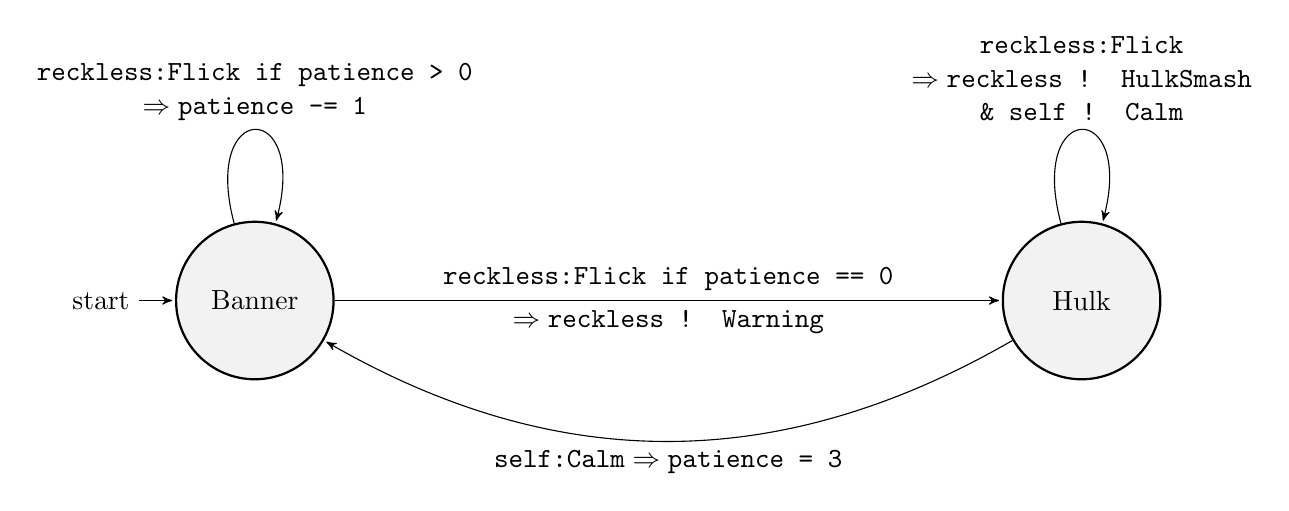
\begin{tikzpicture}[->,>=stealth',
  shorten >=1pt,auto,node distance=2.5cm,
  scale=1,transform shape,align=center,
  state/.style={circle,draw,minimum size=2cm,thick,fill=gray!10}
  ]

  \node[state,initial] (banner) {Banner};
  \node[state,right of=banner,xshift=8cm] (hulk) {Hulk};

  \draw[->] (banner) to
  node[above]
  {$\texttt{reckless:Flick if patience == 0}$}
  node[below]
  {$\Rightarrow \texttt{reckless ! Warning}$}
  (hulk)
  (banner) edge[loop above]
  node {$\texttt{reckless:Flick if patience > 0}$\\$\Rightarrow \texttt{patience -= 1}$}
  (banner)
  (hulk) edge[loop above]
  node {$\texttt{reckless:Flick}$\\$\Rightarrow \texttt{reckless ! HulkSmash}$\\$\texttt{\& self ! Calm}$} (hulk)
  (hulk) edge[bend left, below] node
  {$\texttt{self:Calm} \Rightarrow \texttt{patience = 3}$} (banner);
\end{tikzpicture}
\end{document}